\begin{frame}{Dropout}
    \begin{itemize}
    \item \textbf{Dropout} is a regularization technique used to prevent overfitting in neural networks.
    \item During training, it randomly drops (set to 0) a fraction of neurons in each layer based on a specified probability for every forward pass.
\end{itemize}
    \begin{figure}
    \centering
    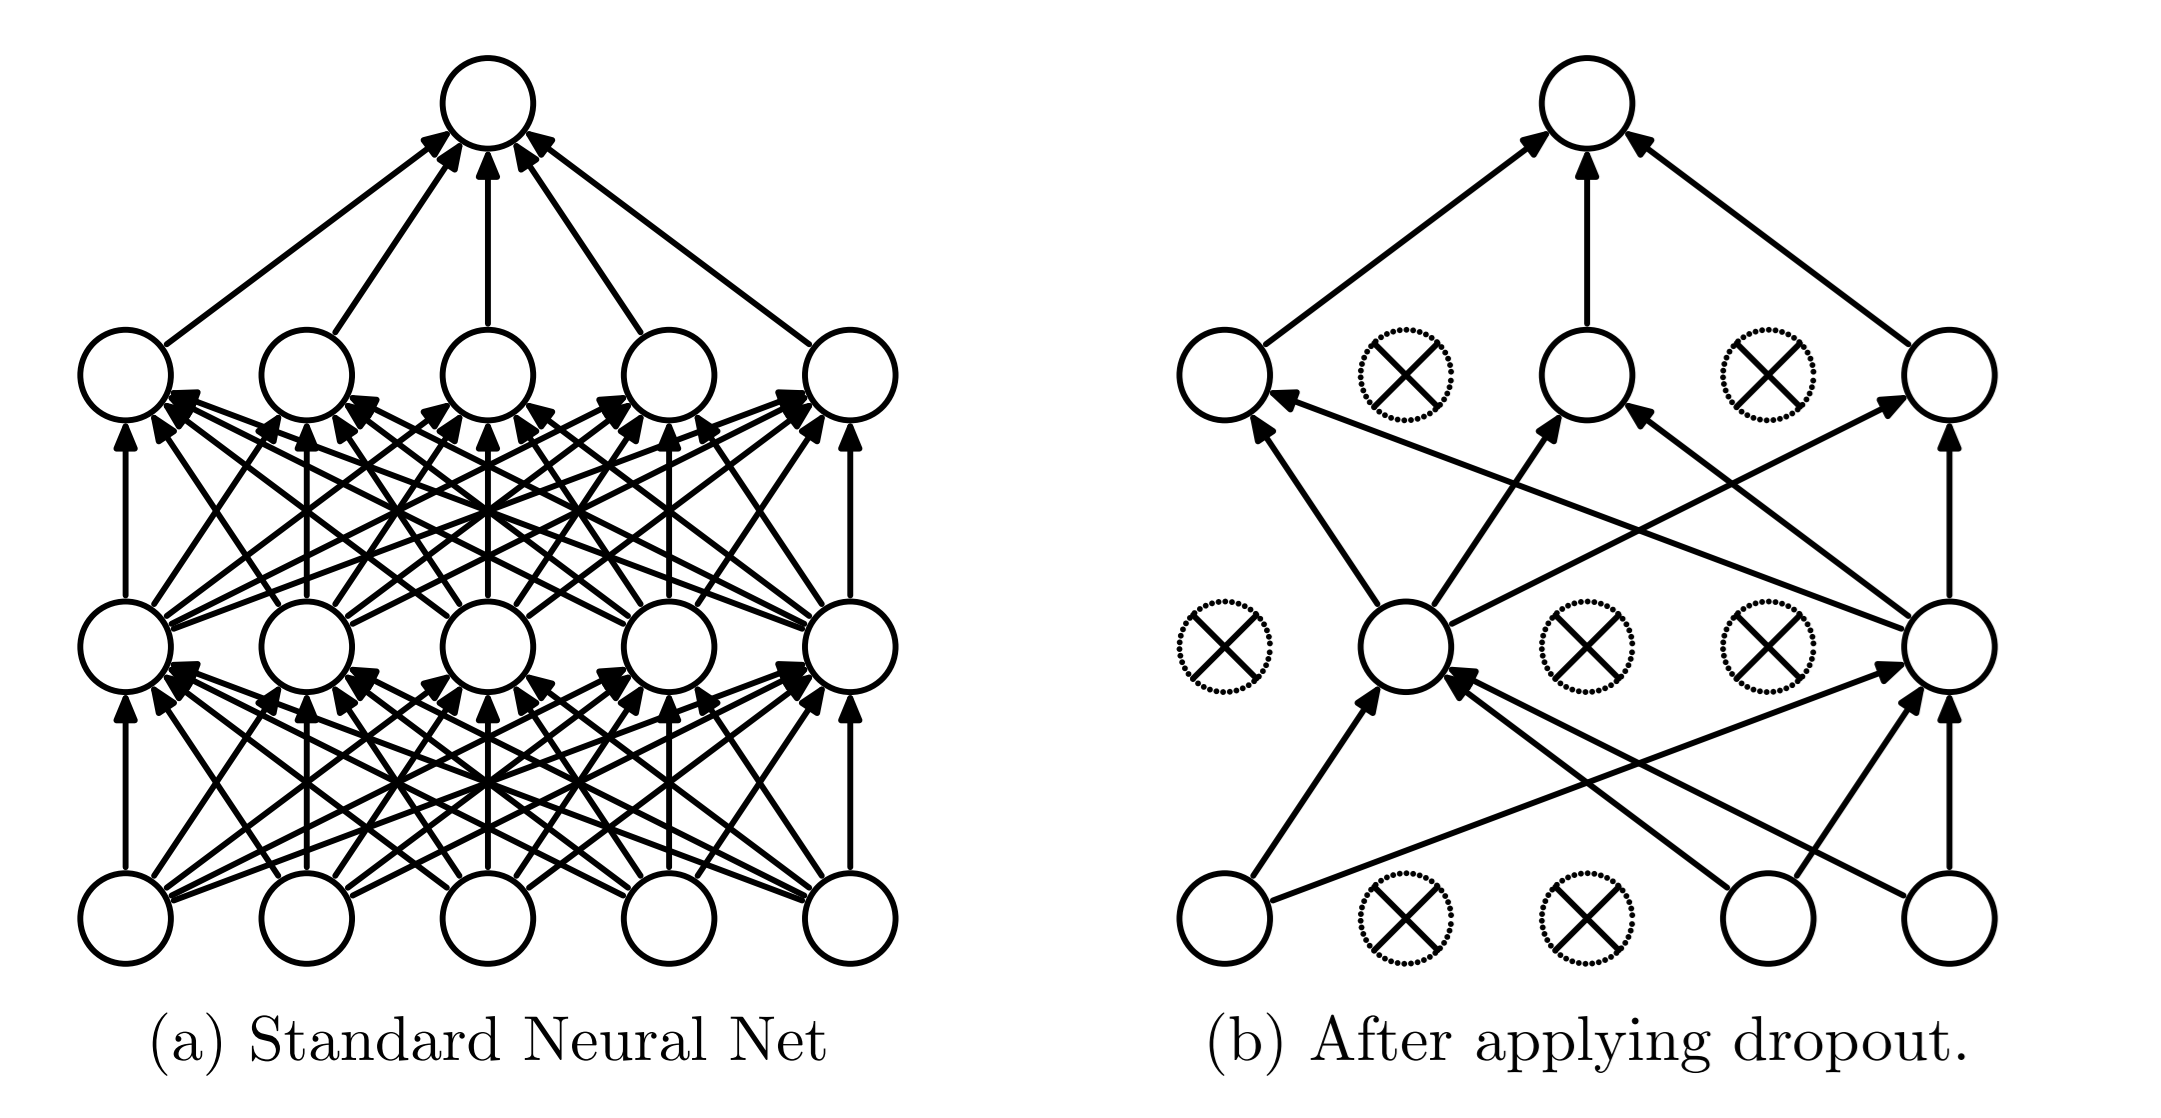
\includegraphics[width=0.8\textwidth,height=0.8\textheight,keepaspectratio]{images/dropout_1.png}
    \end{figure}
\footnotetext{\href{https://jmlr.org/papers/volume15/srivastava14a/srivastava14a.pdf}{Srivastava JMLR 2014}}
\end{frame}

\begin{frame}{Dropout}
\begin{itemize}
    \item Why is dropping neurons randomly useful?
\begin{enumerate}
    \item By dropping a subset of neurons during each forward pass, the network learns \textbf{not to rely too heavily on specific connections}, encouraging the network to use more connections.
    \item Dropout acts as an \textbf{efficient ensemble} of multiple smaller networks, each trained on a random subset of neurons.
    \item More Connections + Diverse Ensemble = \textbf{less overfitting}.
\end{enumerate}
\end{itemize}
\end{frame}

\begin{frame}{Dropout}
    \begin{figure}
    \centering
    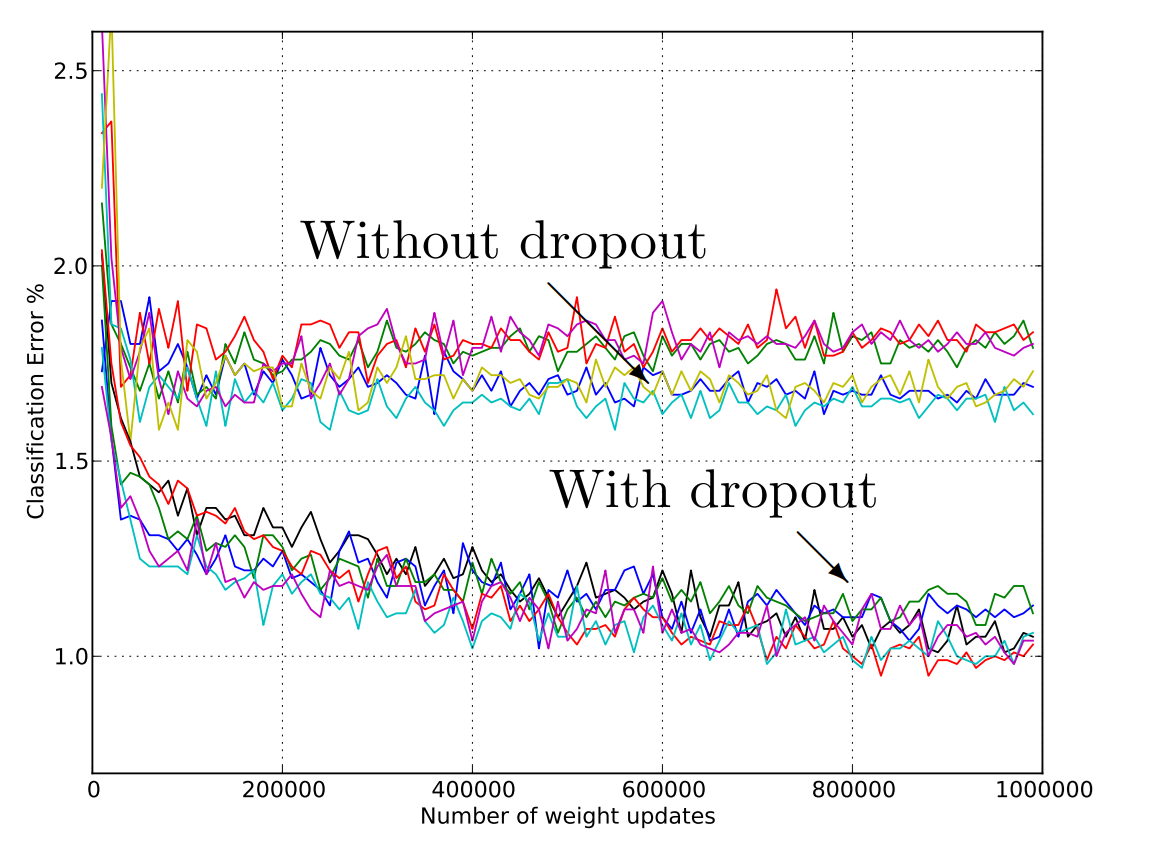
\includegraphics[width=1.0\textwidth,height=0.5\textheight,keepaspectratio]{images/dropout_3.png}
    \end{figure}
    \begin{figure}
    \centering
    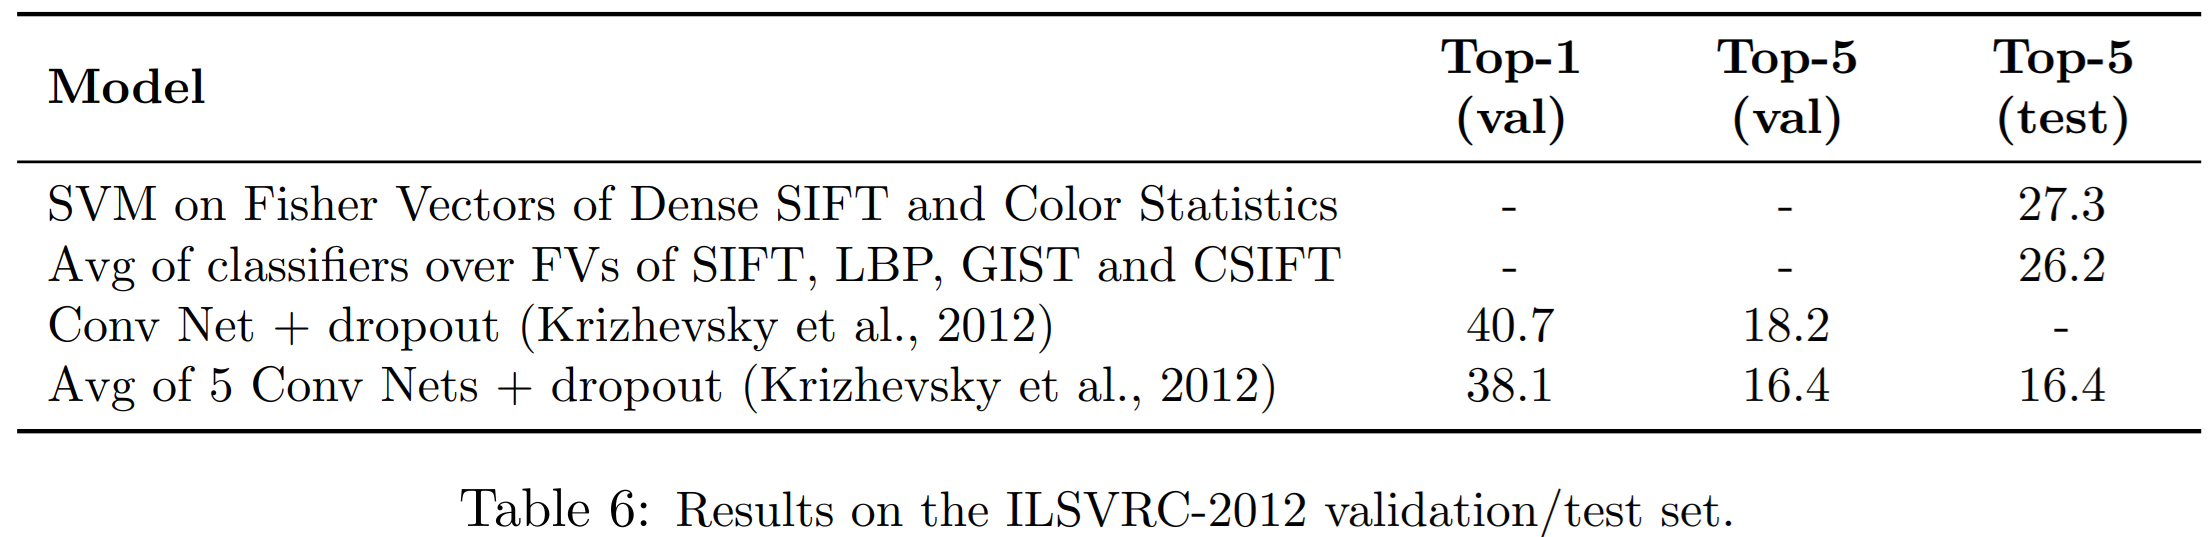
\includegraphics[width=1.0\textwidth,height=0.5\textheight,keepaspectratio]{images/dropout_4.png}
    \end{figure}
\footnotetext{\href{https://jmlr.org/papers/volume15/srivastava14a/srivastava14a.pdf}{Srivastava JMLR 2014}}
\end{frame}

\begin{frame}{Dropout}
\begin{figure}
    \centering
    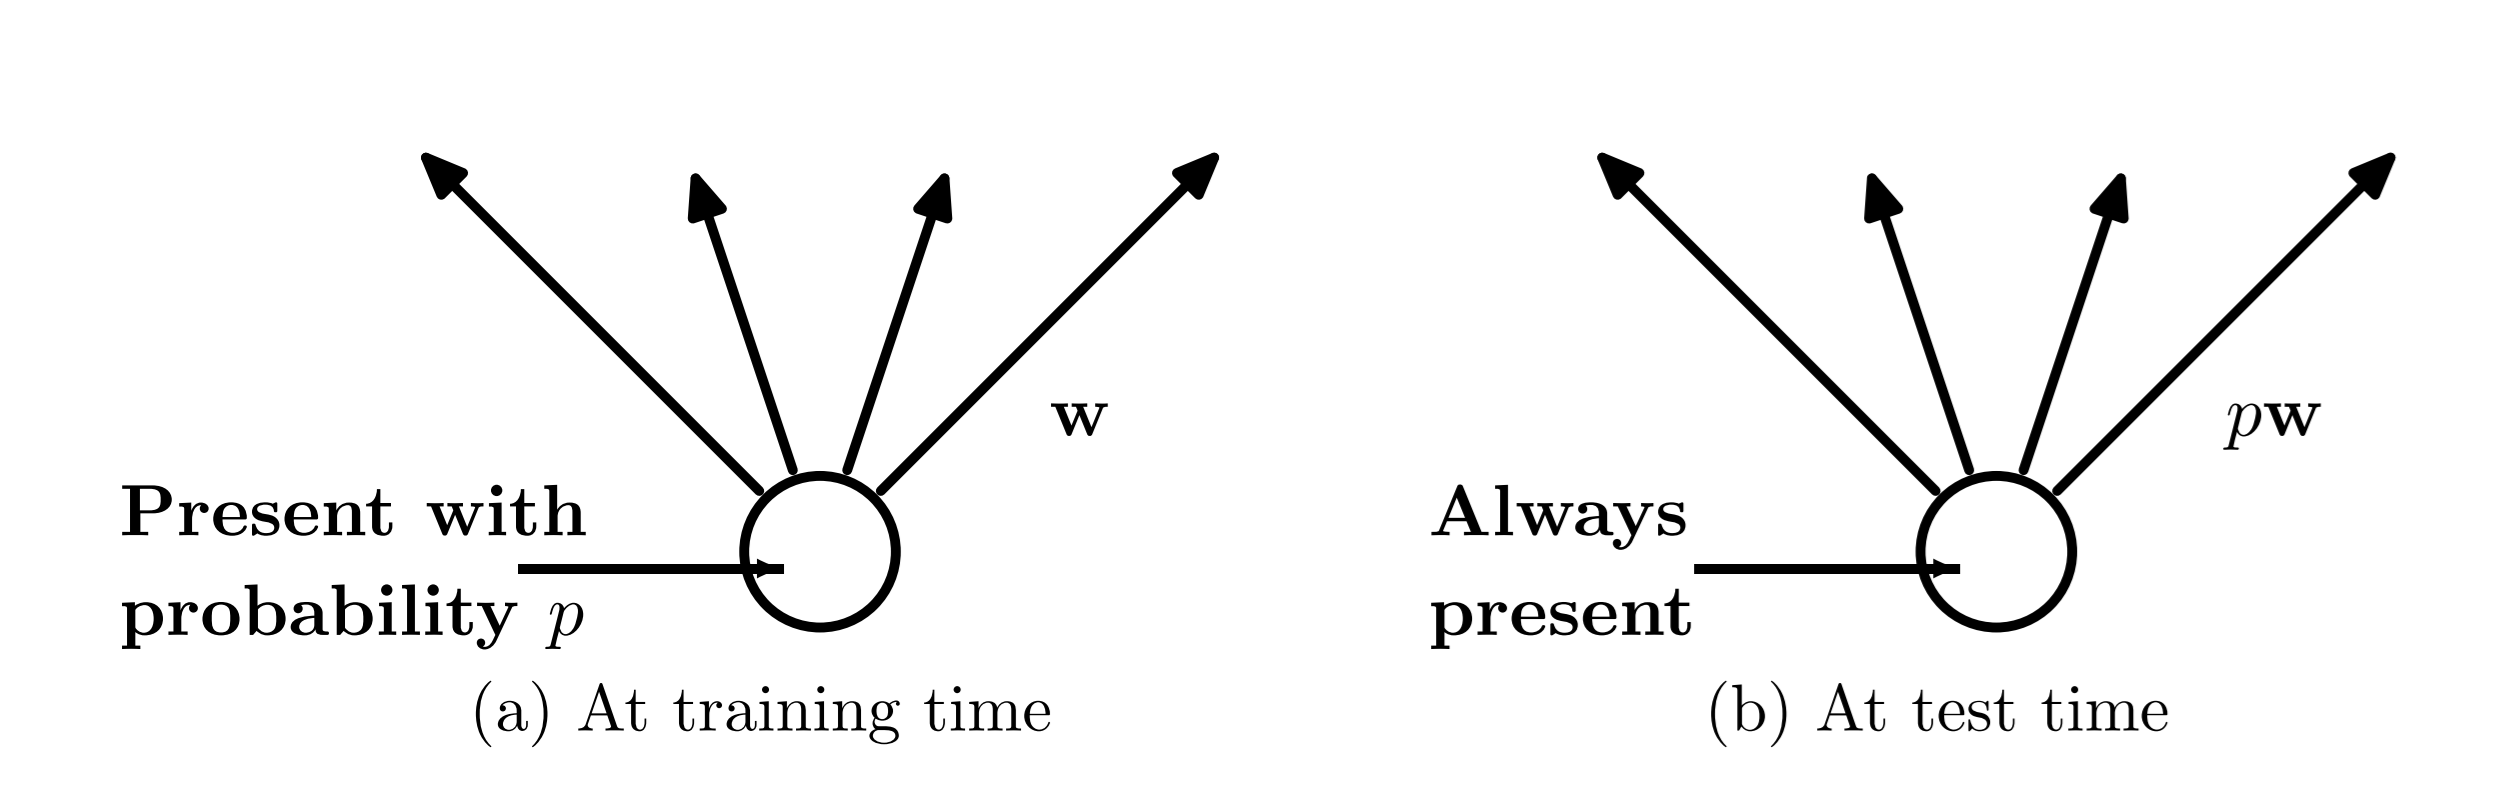
\includegraphics[width=1.0\textwidth,height=0.8\textheight,keepaspectratio]{images/dropout_2.png}
\end{figure}
\begin{itemize}
    \item We drop neurons during training, but what should we do during inference?
    \item \textbf{During inference:} We use all neurons. 
\end{itemize}
But...
\end{frame}

\begin{frame}{Dropout}
\begin{figure}
    \centering
    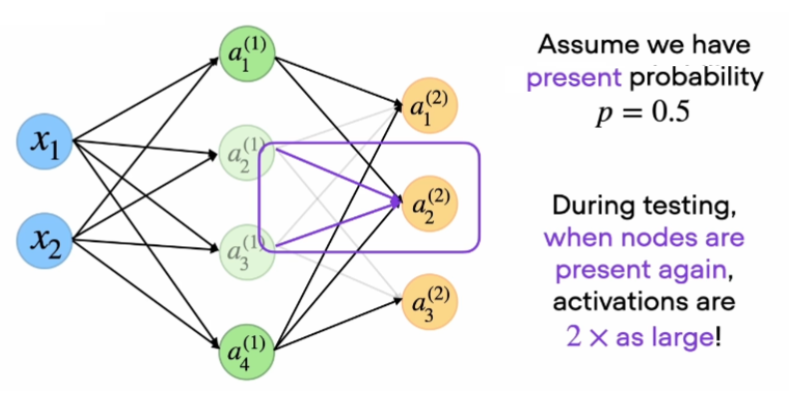
\includegraphics[width=1.0\textwidth,height=1.0\textheight,keepaspectratio]{images/dropout_light.png}
    \end{figure}
    \footnotetext{\href{https://lightning.ai/courses/deep-learning-fundamentals}{Deep Learning Fundamentals - Lightning AI}}
\end{frame}

\begin{frame}{Dropout}
\begin{itemize}
    \item \textbf{Problem:} Having inconsistent values during inference compared to training can cause the network to produce worse results.
    \item \textbf{Solution:} Scale the output during inference by $(p)$ to keep the same expected activation as in training.
    \item \textbf{Example:}
    \begin{itemize}
  \item \textbf{During training (p=0.1)}: 
    \begin{itemize}
      \item Activation value = 2
      \item Active only 10\% of the time 
      \item $\Rightarrow$ Effective contribution = $2 \times 0.1 = 0.2$
    \end{itemize}
  \item \textbf{During inference}: 
    \begin{itemize}
      \item Always active ($\Rightarrow$ Activation value = 2)
      \item Scale by $(p) = 0.1$
      \[
        2 \times 0.1 = 0.2
      \]
    \end{itemize}
  \item Result: Consistent activation scale between training and inference.
\end{itemize}
\end{itemize}
\end{frame}

\begin{frame}{Dropout}
    \begin{itemize}
        \item In PyTorch, dropout behavior is controlled by the model's mode:
            \begin{block}{}
        \texttt{\small
        \# Training Mode: Enables dropout\\
        model.train() \\
        output = model(input) \\
        \\
        \# Evaluation Mode: Disables dropout, scales activations\\
        model.eval() \\
        output = model(input)
        }
    \end{block}
    \end{itemize}
\end{frame} 